\chapter{Vettori Aleatori}

Dopo aver analizzato le proprietà fondamentali delle variabili aleatorie reali, 
in questo capitolo estendiamo la trattazione al caso di vettori aleatori.

\medskip
\noindent L'utilizzo di variabili aleatorie multidimensionali consente di modellare 
fenomeni in cui più quantità casuali interagiscono tra loro, rendendo possibile lo studio delle loro dipendenze, delle distribuzioni congiunte e delle proprietà di indipendenza.\\
\\
Partiremo prima a riassumere le proprietà generali, per poi focalizzarci sui vettori discreti e poi quelli continui.

\begin{definizione}
    $\ve{X}$ è un vettore aleatorio di dimensione $n$ se è una variabile aleatoria in $\mathbb{R}^n$ e 
    \[\ve{X}:(\Omega, \mathcal{A}, \mathbb{P})\to (\mathbb{R}^n, \mathcal{B}^n)\]
\end{definizione}

\begin{teorema}[Ripasso delle Proprietà]
    Per un vettore aleatorio sono valide le seguenti:
    \begin{enumerate}
        \item $\mathcal{B}^n = \underbrace{\mathcal{B}\otimes\cdots\otimes \mathcal{B}}_{n \text{ volte}}$
        \item $\ve{X}$ è misurabile $\quad \iff \quad (X_1, ..., X_n)\;$ sono variabili aleatorie reali
        \item Sia $\ve{X}:\Omega\to\mathbb{R}^n,\;$ e $\;\ve{h}:\mathbb{R}^n\to\mathbb{R}^k$ boreliana \(\qquad \Rightarrow\qquad \ve{Y} = \ve{h}(\ve{X})\; \text{ è un vettore aleatorio in }\;\mathbb{R}^k\)
        \item $\ve{X} \overset{\text{q.c.}}{=}\ve{Y}\quad \iff \quad X_k = Y_k\;\forall k=1, ..., n$
        \item $P^{\ve{X}}\;$ dipende da $\bigl[\ve{X}\bigr]$; ossia che se due vettori sono uguali quasi certamente, allora hanno la stessa legge.
        \item Le componenti $X_1, ..., X_n$ di $\ve{X}$ sono indipendenti $\quad \iff \quad P^{\ve{X}} = \bigotimes_{j = 1}^n P^{X_j}$
        \item $\;X_1, ..., X_n\in L^p(\Omega)\quad \iff\quad \ve{X} \in L^p(\Omega)\;$ 
        \item $X_1, X_2 \in L^2(\Omega, \mathcal{A}, \mathbb{P})\quad \Rightarrow\quad X_1\cdot X_2 \in L^1(\Omega, \mathcal{A}, \mathbb{P})\;\;\text{ e }\;\;\bigl|E[X_1\cdot X_2]\bigr|\leq \sqrt{E[X_1^2]\cdot E[X_2^2]}$
        \item Se $X_1, X_2 \in L^1(\Omega)\;\text{ e }\; X_1\ind X_2\quad \Rightarrow\quad X_1\cdot X_2\in L^1(\Omega)\;\; \text{ e }\;\; E[X_1\cdot X_2] = E[X_1]\cdot E[X_2]$
    \end{enumerate}
\end{teorema}

\section{Vettori Discreti}
Lo studio dei vettori aleatori discreti permette di estendere in modo naturale
i concetti già visti per le variabili discrete — come funzione di massa,
distribuzioni marginali e condizionate, indipendenza e valore atteso —
al caso multidimensionale.
\begin{definizione}
    Dato $(\Omega, \mathcal{A}, \mathbb{P})$ spazio di probabilità, il vettore aleatorio $\ve{X}:\Omega\to\mathbb{R}^n$ è un vettore discreto se $P^{\ve{X}}$ è una probabilità discreta su $\mathcal{B}^n$, ossia che $\exists T\subseteq\mathbb{R}^n$ discreto, ed $\exists \,p_{\ve{X}}:T\to [0, 1]$ tale che:
    \[\sum_{\ve{t}\in T}p_{\ve{X}}(\ve{t}) = 1\qquad \text{e}\qquad P^{\ve{X}}(B) = \sum_{\ve{t}\in T\cap B}p_{\ve{X}}(\ve{t})\quad \forall B\in \mathbb{R}^n\]
\end{definizione}

\begin{teorema}[Condizioni Equivalenti alla 11.3]
\label{th:11.3}
    $\ve{X}$ è un vettore discreto:
    \begin{align*}
        & \iff \quad \exists\,T\subseteq\mathbb{R}\;\text{ discreto tale che }\; \mathbb{P}(\ve{X}\in T) = 1\\
        & \iff \quad \exists\,\ve{Y}\;\text{ con Im}(Y)=T\;\text{ tale che }\; \ve{X}\overset{\text{q.c.}}{=}\ve{Y}\\
        & \iff \quad X_1, ..., X_n\;\text{ sono variabili aleatorie discrete, ovvero che }\;P^{X_k}\;\text{ è discreto }\;\forall k=1, ..., n
    \end{align*}
    \begin{dimostrazione}
        Dimostriamo solo la terza implicazione in direzione $(\Leftarrow)$.\\
        Per dimosrtare che dati $X_k$ discreto con $S_{X_k}$ il suo supporto $\;\forall k=1, ..., n$ ci basta trovare un $T\subseteq\mathbb{R}^n\;$ tale che $\;\mathbb{P}(\ve{X}\in T)=1$.

        \medskip
        \noindent Per avere un'idea grafica di cosa significhi questo, mettiamoci nel caso semplice in cui abbiamo solo $X_1, X_2$ e quindi $T=S_{X_1}\times S_{X_2}, \;$ dove $S_{X_1} = \{1, 2, 3\};\;S_{X_2} = \{\frac{1}{2}, \frac{3}{2}\}$.
        \begin{figure}[H]
\centering
\begin{tikzpicture}[scale=1, >=stealth, font=\small]

% --- Assi ---
\draw[->, thick] (0,0) -- (3.8,0) node[right] {$X_1$};
\draw[->, thick] (0,0) -- (0,2.5) node[above] {$X_2$};
\node[below, red] at (3.1,2.5) {$T$};
% --- Tacche sugli assi ---
\foreach \x in {1,2,3}{
  \draw[fill=black] (\x,0) circle (1pt);
  \node[below] at (\x,0) {$\x$};
}
\foreach \y/\label in {0.5/{$\tfrac{1}{2}$}, 1.5/{$\tfrac{3}{2}$}}{
  \draw[fill=black] (0,\y) circle (1pt);
  \node[left] at (0,\y) {\label};
}

% --- Linee tratteggiate grigie (coordinate dei punti) ---
\foreach \x in {1,2,3}{
  \foreach \y in {0.5,1.5}{
    \draw[dashed, gray!60] (\x,0) -- (\x,\y);
    \draw[dashed, gray!60] (0,\y) -- (\x,\y);
  }
}

% --- Punti discreti rossi ---
\foreach \x in {1,2,3}{
  \foreach \y in {0.5,1.5}{
    \fill[red] (\x,\y) circle (2pt);
  }
}

\end{tikzpicture}
\end{figure}

    Ovviamente per $n$ componenti si estende a $T=S_{X_1}\times \cdots \times S_{X_n}$.\\
    Dunque: 
    \begin{align*}
        \mathbb{P}(\ve{X}\in T) & = \mathbb{P}(\ve{X} \in S_{X_1}\times \cdots \times S_{X_n}) = \mathbb{P}(X_1\in S_{X_1}, ..., X_n\in S_{X_n}) \\
        & = \mathbb{P}\left( \bigcap_{k=1}^n \bigl(X_k \in S_{X_k}\bigr)\right) \overset{\text{De Morgan}}{ = }1- \mathbb{P}\left(\bigcup_{k=1}^n (X_k\in S_{X_k})^c\right)\\
        & = 1- \underbrace{\sum_{k=1}^n\mathbb{P}(X_k\notin S_{X_k})}_{0} = 1
    \end{align*}
    \end{dimostrazione}
\end{teorema}

\begin{proposizione}
    Sia $\ve{X}$ un vettore aleatorio discreto $n$--dimensionale con $T = T_1\times\cdots\times T_n$.\\
    Allora vale che:
    \begin{enumerate}
        \item Per la regola del valore atteso:
        \[E[h(\ve{X})] = \int_\Omega h(\ve{X})\;d\mathbb{P} = \int_{\mathbb{R}^n}h(\ve{t})\;dP^{\ve{X}} = \sum_{\ve{t}\in T} h(\ve{t})\,p_{\ve{X}}(\ve{t})\]
        Dove: \(\qquad h\in L^1(P^{\ve{X}})\quad \iff \quad\sum_{\ve{t}\in T} \bigl|h(\ve{t})\,p_{\ve{X}}(\ve{t})\bigr| <+\infty \)
        \item Il rapporto tra la legge congiunta, e le marginali è il seguente:
        \[p_{X_k}(t_k) = \sum_{t_1\in T_1; \cdots; t_{k-1}\in T_{k-1};t_{k+1}\in T_{k+1};\cdots; t_n\in T_n}p_{\ve{X}}(t_1, ..., t_k, ..., t_n)\]
        \item $X_1, ..., X_n\;$ sono indipendenti\footnote{D'ora in avanti si utilizzerà un piccolo abuso di notazione: scriveremo che ``$X_1, ..., X_n$ sono indipendenti'' per intendere che siano una famiglia di V.A. indipendenti. Non è sufficiente infatti che $X_1, ..., X_n$ siano indipendenti a coppie, ma vi è la necessità che seguano la definizione di famiglia di V.A. indipendenti.} $\quad \iff \quad p_{\ve{X}} (t_1, ..., t_n) = p_{X_1}(t_1)\cdots p_{X_n}(t_n)\quad \forall \ve{t}\in T$
    \end{enumerate}
\end{proposizione}

È importante notare che il secondo punto ci dice come possiamo calcolare una legge marginale a partire dalla congiunta. Per ottenere la legge di $X_k$ è infatti sufficiente fissare il valore di $X_k$ e fare la somma della legge congiunta su tutte le altre componenti del vettore.

\begin{esempio}
    Per intenderci mettiamoci nel caso in cui $n=2$. Consideriamo due variabili aleatorie discrete $(X_1, X_2)$, con
    \[
        T_1 = \{1,2,3\}, \qquad T_2 = \{a,b\},
    \]
    e legge congiunta data dalla seguente tabella:
    \[
    \begin{array}{c|cc}
        & X_2 = a & X_2 = b \\ \hline
        X_1 = 1 & 0.1 & 0.2 \\
        X_1 = 2 & 0.3 & 0.1 \\
        X_1 = 3 & 0.2 & 0.1
    \end{array}
    \]

    La legge marginale di $X_1$ si ottiene sommando la probabilità congiunta su tutti i possibili valori di $X_2$:
    \[
        p_{X_1}(t_1) = \sum_{t_2 \in T_2} p_{\ve{X}}(t_1, t_2).
    \]
    In particolare:
    \[
    \begin{aligned}
        p_{X_1}(1) &= p_{\ve{X}}(1,a) + p_{\ve{X}}(1,b) = 0.1 + 0.2 = 0.3,\\
        p_{X_1}(2) &= p_{\ve{X}}(2,a) + p_{\ve{X}}(2,b) = 0.3 + 0.1 = 0.4,\\
        p_{X_1}(3) &= p_{\ve{X}}(3,a) + p_{\ve{X}}(3,b) = 0.2 + 0.1 = 0.3.
    \end{aligned}
    \]
    Quindi la legge marginale di $X_1$ risulta:
    \[
        p_{X_1} : T_1 \to [0,1]: \qquad
        p_{X_1}(1) = 0.3, \quad p_{X_1}(2) = 0.4, \quad p_{X_1}(3) = 0.3.
    \]
\end{esempio}
\begin{esempio}
    Prendiamo come esperimento il lancio di 3 dadi, sia quindi $\ve{X} = (X_1, X_2, X_3)$ e sia $X_K=\text{ Risultato del $k$--esimo dado}$.\\
    Grazie al Teorema \ref{th:11.3} possiamo dire che $\ve{X}$ è un vettore aleatorio discreto, in quanto le sue componenti sono V.A. discreto. Inoltre, per ragioni modellistiche le $X_1, X_2, X_3$ risultano essere indipendenti, e quindi:
     \[p_{\ve{X}}(h_1, h_2, h_3) = p_{X_1}(h_1)\cdot p_{X_2}(h_2)\cdot p_{X_3}(h_3)\qquad \forall h_k\in\{1, ...,6\}, k=1, 2, 3\]
     Quindi per esempio: $\quad p_{\ve{X}}(1, 1, 1) = p_{X_1}(1)\cdot p_{X_2}(1)\cdot p_{X_3}(1) = \frac{1}{6^3}$.

     \medskip
     \noindent Definiamo ora $Y:=X_1+X_2$, la quale risulta essere discreta perché somma di discrete. Siccome possiamo vedere $Y$ come $Y = h(X_1, X_2)$, allora è evidente che $Y\ind X_3$, siccome $(X_1, X_2)\ind X_3$.
     
     \medskip
     \noindent Consideriamo ora il vettore $(X_1, Y)^\top$ discreto, in quanto ha componenti discrete. Ci chiediamo a questo punto, \textit{$X_1$ e $Y$ sono indipendenti?}\\
     \\
     Siccome conosciamo le marginali possiamo andare a calcolare la congiunta, di seguito una tabella che riassume i risultati:

\begin{table}[H]
\centering
\small
\renewcommand{\arraystretch}{1.2}
\[
\begin{array}{c|ccccccccccc|c}
X_1\backslash Y & 2 & 3 & 4 & 5 & 6 & 7 & 8 & 9 & 10 & 11 & 12 & p_{X_1}(x)\\ \hline
1 & 1/36 & 1/36 & 1/36 & 1/36 & 1/36 & 1/36 & 0 & 0 & 0 & 0 & 0 & 1/6\\
2 & 0 & 1/36 & 1/36 & 1/36 & 1/36 & 1/36 & 1/36 & 0 & 0 & 0 & 0 & 1/6\\
3 & 0 & 0 & 1/36 & 1/36 & 1/36 & 1/36 & 1/36 & 1/36 & 0 & 0 & 0 & 1/6\\
4 & 0 & 0 & 0 & 1/36 & 1/36 & 1/36 & 1/36 & 1/36 & 1/36 & 0 & 0 & 1/6\\
5 & 0 & 0 & 0 & 0 & 1/36 & 1/36 & 1/36 & 1/36 & 1/36 & 1/36 & 0 & 1/6\\
6 & 0 & 0 & 0 & 0 & 0 & 1/36 & 1/36 & 1/36 & 1/36 & 1/36 & 1/36 & 1/6\\ \hline
p_Y(y) & 1/36 & 2/36 & 3/36 & 4/36 & 5/36 & 6/36 &
5/36 & 4/36 & 3/36 & 2/36 & 1/36 &
\end{array}
\]
\end{table}

Si vede che $X_1$ e $Y$ non sono indipendenti, perché per esempio $p_{(X_1, Y)}(2, 2) \neq p_{X_1}(2)\,p_{X_2}(2)$
\end{esempio}

\section{Vettori Assolutamente Continui}
La trattazione dei vettori assolutamente continui, come vedremo, sarà inevitabilmente più complessa e meno lineare rispetto a quelli discreti.\\
\\
Ricordiamo la definizione della misura di Lebesgue $n$--dimensionale già esposta a pagina \pageref{leb_ndim}:
\[m_n = \bigtimes_{j=1}^n[a_j, b_j) = \prod_{k=1}^n(b_k-a_k)\]

\medskip
\noindent Dovremo inizialmente allargare le definizioni esposte nel caso monodimensionale al caso multidimensionale. Iniziamo dalla definizione di probabilità continua (Definizione \ref{def:9.1}).

\begin{definizione}
\label{def:11.6}
    Una misura di probabilità $\mathbb{P}$ su $\mathcal{B}(\mathbb{R}^n)$ si dice assolutamente continua se
    \[\exists\,f:\mathbb{R}^n\to \mathbb{R}^+\]
    boreliana, definita \textit{densità continua}, tale che $\;\forall A\in \mathcal{B}(\mathbb{R}^n):$
    \[\mathbb{P}(A) = \int_Af(\ve{x})\;dm_n = \int_{\mathbb{R}^n} f\cdot \mathbb{I}_A\;dm_n = \int_{\mathbb{R}^n} f(\ve{x})\cdot\mathbb{I}_A(\ve{x})\;d\ve{x}\]
\end{definizione}

Si osservi che se $n=1$, allora la Definizione \ref{def:11.6} è equivalente alla Definizione \ref{def:9.1} tramite funzione di ripartizione.

\begin{definizione}
    $\ve{X}:\Omega\to\mathbb{R}^n$ è un Vettore Aleatorio Assolutamente Continuo se $P^{\ve{X}}$ è una misura di probabilità su $(\mathbb{R}^n, \mathcal{B}(\mathbb{R}^n))$ assolutamente continua, e denotiamo la densità congiunta del vettore $\ve{X}$ con $f_{\ve{X}}$
\end{definizione}

\begin{teorema}[Caratterizzazione di una Densità Continua]
Valgono i seguenti:
\begin{enumerate}
\label{th:11.9}
    \item $f:\mathbb{R}^n\to\mathbb{R}$ è una densità continua congiunta di una probabilità $\mathbb{P}$ assolutamente continua su $\mathcal{B}^n$ \underline{se e solo se}:
    \begin{enumerate}
        \item $f$ è Boreliana
        \item $f\geq0$
        \item $\int_{\mathbb{R}^n}f(x)\;dx = 1$
    \end{enumerate}
    \item Se vale (1.), allora:
    \[\mathbb{P}(A) = \int_Af\;dm_n = \int_A f(x)\;dx\quad \forall A\in \mathcal{B}(\mathbb{R}^n)\]
    \item $\mathbb{P}$ su $\mathcal{B}(\mathbb{R}^n)$ assolutamente continua è univocamente caratterizzata dalla classe di equivalenza della sua densità continua $[f]$, ossia:
    \[f_1=f_2\;\;m_n\text{--quasi ovunque}\quad \iff \quad \mathbb{P}_1 = \mathbb{P}_2\]
\end{enumerate}
\end{teorema}

\begin{esempio}
    Si vuole modellizzare da un punto di vista probabilistico il gioco delle freccette. Sia $C$ l'insieme dove viene lanciata a caso la freccetta, definito come
    \[C = \set{(x, y)\in\mathbb{R}^2\mid x^2+y^2\leq1}\]
    e sia rappresentino le coordinate del lancio con il vettore $(X, Y)$. Vogliamo trovare $f_{(X, Y)}$ densità assolutamente continua.

    \medskip
    \noindent Il fatto che il lancio venga effettuato a caso all'interno del cerchio, ci fa intuire che potremmo essere davanti ad una densità uniforme, del tipo:
    \[f_{(X, Y)}(x, y) = c\cdot \mathbb{I}_C(x, y)\]
    Allora per il Teorema \ref{th:11.9}, affinché sia una densità continua devono valere le tre condizioni del punto 1.
    \[\Rightarrow\qquad \begin{cases}
        f \text{boreliana}\quad &\Rightarrow \quad f \text{\; è boreliana}\\
        f\geq0 \quad &\Rightarrow \quad c\geq 0\\
        \int_{\mathbb{R}^n} c\cdot \mathbb{I}_C(x, y)\;dxdy = 1 \quad &\Rightarrow \quad c\cdot m_2(C) = c\pi 1^2 \quad \Rightarrow \quad c = 1/\pi
    \end{cases}\]
    Questo basta per dire che $\;f_{(X, Y)}(x, y) = \frac{1}{\pi}\,\mathbb{I}_C(x, y)\;$ è una densità congiunta assolutamente continua.
\end{esempio}

Si osservi che preso un $A\in \mathcal{B}^n$ tale che $m_n(A)=0$ e $\mathbb{P}$ è una misura di probabilità assolutamente continua su $\mathcal{B}^n$, allora:

\[\mathbb{P}(A) = \int_{\mathbb{R}^n} \mathbb{I}_A(x)\,f(x)\;dx = 0, \quad \text{ siccome }\quad \mathbb{I}_A=0 \;\text{ q.o.}\]

\noindent Questo vuol dire, per esempio, che se siamo su $\mathbb{R}^2$, la retta ha misura nulla: un vettore in $\mathbb{R}^2$ ha probabilità $0$ di prendere valori su una retta.

\(\Rightarrow\qquad\;\) Se $A$ è un sottospazio di dimensione $\leq n-1, \;$ allora $m_n(A) = 0$

\begin{esempio}
    Si prenda:
    \[
        g:\mathbb{R}\to\mathbb{R}, \qquad g(x) = x^2
    \]
    Allora il Grafico $G$ definito come
    \[G=\set{\bigl(x, g(x)\bigr)=(x, x^2)\in\mathbb{R}^2\mid x\in\mathbb{R}^2}\]
    Avrà misura di Lebesgue $2$--dimensionale nulla: $\quad m_2(G)=0$
\end{esempio}
\(\Rightarrow\quad\) Anche i grafici hanno misura nulla: $\quad m_n(G) = 0$.
\begin{esempio}[\faWarning]
    Vediamo con un esempio, una caratteristica fondamentale dei vettori assolutamente continui. Si consideri:
    \[X\sim \mathcal{E}(\lambda), \;\lambda >0;\qquad f_X(t) = \lambda e^{-\lambda t}\;\mathbb{I}_{(0, +\infty)}(t)\]
    Ovviamente $X$ è assolutamente continuo, ma anche $X^2$ lo è, difatti\footnote{Trovata sapendo che: $F_{X^2}(t) = \mathbb{P}(-\sqrt{t}\leq X\leq \sqrt{t}) = F_X(\sqrt{t})-F_X(-\sqrt{t})\quad \Rightarrow\quad f_{X^2}(t) = \frac{d}{dt}\left(F_{X^2}(t)\right) = \frac{f_X(\sqrt{t})-f_X(-\sqrt{t})}{2\sqrt{t}}$}:
    
    \[f_{X^2}(t) = \frac{\lambda e^{-\lambda \sqrt{t}}}{2\sqrt{t}}\;\mathbb{I}_{(0, +\infty)}(t)\]
    Componendo il vettore $(X, X^2)^\top$, ci chiediamo: \textit{posso dedurre che il vettore sia assolutamente continuo, dato che le sue componenti sono assolutamente continue (come è lecito fare nel caso discreto)?} Ossia:
    \[\exists?\,f_{(X, X^2)}:\mathbb{R}^2\to\mathbb{R}\quad \text{ tale che }\quad  P^{(X, X^2)}(A) = \int_Af_{(X, X^2)}\;d\ve{x}\;?\]
    La risposta è \textbf{assolutamente no}. Infatti:
    \[\text{Im}(X, X^2) = \set{(x, x^2)\in\mathbb{R^2}\;:\;x\in\mathbb{R}} = G\]
    Di conseguenza:
    \[\mathbb{P}((X, X^2)\in G) = 1\qquad \Rightarrow\qquad P^{(X, X^2)}(G) = 1\]
    Ma noi sappiamo dall'esempio precedente che $m_2(G) = 0$, e quindi dovrebbe essere (se il vettore fosse continuo) che $P^{(X, X^2)}(G) = 0$
\end{esempio}

Abbiamo appena dimostrato con un esempio che \textbf{non basta che le componenti del vettore siano separatamente continue per concludere che il vettore stesso sia assolutamente continuo}, ossia che esista una densità congiunta.

\begin{teorema}
    Sia $\ve{X} = (X_1, ..., X_n)$ un vettore assolutamente continuo, allora valgono che:
    \begin{enumerate}
        \item $h\in L^1(P^X)\quad \iff \quad h\cdot f_{\ve{X}}\in L^1(m_n) \quad \iff \quad \int_{\mathbb{R}^n}\bigl|h(\ve{x})\bigr|\,f_{\ve{X}}(\ve{x})\;d\ve{x}<+\infty$. 

        \medskip
        \noindent Allora, se vale una delle precedenti oppure se $h\geq0$, si ha per la regola del valore atteso che:
        \[\boxed{E\bigl[h(\ve{X})\bigr] = \int_{\mathbb{R}^n} h\;dP^{\ve{X}} = \int_{\mathbb{R}^n}h(\ve{x})\,f_{\ve{X}}(\ve{x})\;d\ve{x}}\]
        \item Ogni $X_k:(\Omega, \mathcal{A}, \mathbb{P})\to (\mathbb{R}, \mathcal{B}(\mathbb{R}))$ è una variabile aleatoria assolutamente continua, con densità
        \[f_{X_k}(x_k) = \int_{\mathbb{R}^{n-1}}f_{\ve{X}}(x_1, ..., x_n)\;dx_1\cdots dx_{k-1}dx_{k+1}\cdots dx_n\]
        \item $(X_1, ..., X_n)$ formano una famiglia di V.A. indipendenti assolutamente continue, con densità marginali $f_{X_1}, ..., f_{X_n}$
        \[\iff \quad \ve{X}\;\text{ è assolutamente continuo }\quad \text{e}\quad f_{\ve{X}}(x_1, ..., x_n) = f_{X_1}(x_1)\cdots f_{X_n}(x_n)\quad \text{quasi ovunque}\]
    \end{enumerate}
\end{teorema}

Si può cercare di dare un'intuizione grafica al punto 2. di quest'ultimo teorema, almeno nel caso bidimensionale. Ipotizziamo di avere una densità $f_{(X_1, X_2)}$, allora la legge marginale di $X_1$ può essere calcolata come
\[f_{X_1}(x_1)=\int_{\mathbb{R}} f_{(X_1,X_2)}(x_1,x_2)\,dx_2\]

\begin{figure}[H]
\centering
\begin{tikzpicture}
\begin{axis}[
    view={60}{28},
    domain=-3:3, y domain=-3:3,
    samples=45, samples y=45,
    xlabel={$x_1$}, ylabel={$x_2$}, zlabel={$f_{(X_1,X_2)}(x_1,x_2)$},
    ylabel style={
         rotate=0,          % <-- ruota l'etichetta in orizzontale
         anchor=north east, % <-- opzionale: regola l'ancoraggio per non farla sovrapporre
         yshift=-2pt        % <-- opzionale: piccolo aggiustamento verticale
    },
    zmin=0, zmax=0.35,      % <-- abbastanza alto per la marginale
    colormap/viridis,
    grid=major,
    axis lines=box,
    clip=false,             % <-- evita il taglio di linee/etichette
    ticklabel style={font=\small},
    label style={font=\small},
    z buffer=sort
]

% --- Superficie congiunta N(0, I) 2D
\addplot3[surf, shader=interp]
{ (1/(2*pi)) * exp(-0.5*(x^2 + y^2)) };

% --- Curva sul pavimento (profilo gaussiano lungo x1, solo decorativa)
\addplot3[thick, gray!70, domain=-3:3, samples=50]
({x}, { -3 }, { 0 }); % profilo a z=0

% --- Marginale esatta f_{X1}(x1) = (1/sqrt(2pi)) e^{-x1^2/2} a x2=-2.8
\addplot3[very thick, red, domain=-3:3, samples=50]
({x}, {-2.8}, {(1/sqrt(2*pi))*exp(-0.5*x^2)});
\node[red,anchor=west] at (axis cs:1.2,-2.8,0.33) {$f_{X_1}(x_1)$};

% --- Sezione a x1 = xbar: si integra lungo x2
\def\xbar{1.2}
\addplot3[dashed, thick, gray] coordinates {(\xbar,-3,0) (\xbar,3,0)};
\addplot3[thick, gray, domain=-3:3, samples=50]
({\xbar}, {y}, {(1/(2*pi))*exp(-0.5*(\xbar*\xbar + y*y))});
\node[gray!70!black, anchor=west, fill=white, text opacity=1]
    at (axis cs:\xbar,2.3,0.1)
    {integra in $x_2$};

\end{axis}
\end{tikzpicture}
\end{figure}


Dal punto di vista grafico, la legge congiunta gaussiana può essere rappresentata come una \emph{superficie tridimensionale} sul piano $(x_1,x_2)$, la cui altezza in ciascun punto rappresenta il valore della densità $f_{X_1,X_2}(x_1,x_2)$. 

\medskip
Graficamente, $f_{X_1}$ corrisponde a \emph{proiettare la superficie tridimensionale} 
sull'asse $x_1$, ``collassando'' la seconda dimensione. 
In altre parole, per ogni valore fissato di $x_1$ si sommano 
(le aree sotto la curva in direzione $x_2$) tutti i contributi di probabilità
associati ai diversi valori di $x_2$. Il risultato è una \emph{curva bidimensionale} 
lungo l'asse $x_1$, che rappresenta la densità marginale $f_{X_1}(x_1)$.\\
\\
In sintesi, la densità congiunta descrive come la probabilità si distribuisce 
nell'intero piano $(x_1,x_2)$, mentre la densità marginale rappresenta 
la ``proiezione'' di tale distribuzione su uno dei due assi, ottenuta 
attraverso un'operazione di integrazione.

\begin{teorema}
    Siano $\;X_1:(\Omega, \mathcal{A}, \mathbb{P})\to (\mathbb{R}^n, \mathcal{B}^n), \;X_2:(\Omega, \mathcal{A}, \mathbb{P})\to (\mathbb{R}^k, \mathcal{B}^k) \quad $ vettori aleatori assolutamente continui, ossia che esistono $f_{X_1}, f_{X_2}$. Supponiamo inoltre che $X_1\ind X_2$:\\
    \(\Rightarrow\quad \ve{X}\; \text{ è un vettore assolutamente continuo con densità:}\)
    \[f_{\ve{X}} = (x_1, ..., x_n, y_1, ...y_k) = f_{X_1}(x_1, ..., x_n)\cdot f_{X_2}(y_1, ..., y_k) \quad \forall (x_1, ..., x_n, y_1, ..., y_k)\in \mathbb{R}^{n+k}\]
\end{teorema}

\begin{esempio}
    Sia $\begin{bmatrix}
        X\\Y
    \end{bmatrix}$ un vettore assolutamente continuo con densità:
    \[f_{(X, Y)} (x, y) = \frac{1}{\pi}\cdot\mathbb{I}_C(x, y)\]
    Ci chiediamo quali siano le densità marginali, e se $X, Y$ siano indipendenti.\\
    Posso calcolare la marginali come:
    
    \begin{align*}
        &f_X(x) = \int_\mathbb{R}f_{(X, Y)}(x, y)\;dy = \begin{cases}
        0, \quad  &|x|>1\\
        \frac{2\sqrt{1-x^2}}{\pi} \quad  -1<&x<1
    \end{cases} = \frac{2\sqrt{1-x^2}}{\pi} \mathbb{I}_{[-1, 1]}(x)\\
    &f_Y(y) = \frac{2\sqrt{1-y^2}}{\pi} \mathbb{I}_{[-1, 1]}(y)
    \end{align*}

    \bigskip
    Siccome $f_{(X, Y)}$ risulta essere diverso da zero su un cerchio, mentre $f_X(x) \cdot f_Y(y)$ è diverso da zero su di un quadrato, allora sicuramente $X, Y$ non possono essere indipendenti.
\end{esempio}

\bigskip
\noindent
\begin{tikzpicture}
  \draw[dashed] (0,0) -- (\textwidth,0);
\end{tikzpicture}\\
\\
Facciamo un \textbf{breve riassunto pratico}.\\
\\
Nel caso in cui sia dato $\ve{X}$ assolutamente continuo, e si definisca $\ve{Y}:=h(\ve{X})$, allora ci sono 3 casistiche nelle quali possiamo ritrovarci:
\begin{enumerate}
\label{riassunto_pratico}
    \item Se $h$ ha immagine discreta $\quad \Rightarrow \quad \ve{Y}$ è una V.A. discreta.
    \begin{esempio}
        Un classico esempio già visto è il caso in cui $\ve{Y}=h(\ve{X})=[\ve{X}]$
    \end{esempio}
    \item Se $h\in C^1\;$ tale che $\;h^{-1}\in C^1 \quad \Rightarrow \quad \ve{Y}$ è una V.A. assolutamente continua, e vale che:
    \[f_{\ve{Y}}(\ve{y})=f_{\ve{X}}(h^{-1}(\ve{y}))\cdot \bigl|\det J_{h^{-1}}(y)\bigr|\]
    \item Ne continua, ne discreta: un Troll di Montagna.
    \begin{esempio}
        Un classico esempio è il caso in cui $\ve{Y}=h(\ve{X})=\ve{X}^2$
    \end{esempio}
\end{enumerate}

\bigskip
\section{Covarianza}
La covarianza è un indice che misura come due variabili aleatorie si muovono congiuntamente rispetto ai rispettivi valori medi. In altre parole, essa descrive la tendenza delle due variabili a variare insieme.

\medskip
Dal punto di vista concettuale, la covarianza può essere vista come
un'estensione della varianza al caso di due variabili aleatorie:
mentre la varianza misura la dispersione di una singola variabile
rispetto alla propria media, la covarianza quantifica la
\emph{dipendenza} tra due variabili, cioè quanto le loro variazioni risultano correlate.\\
\\
Diamo quindi la definizione formale:
\begin{definizione}
    Sia $\begin{bmatrix}X\\Y\end{bmatrix}:(\Omega, \mathcal{A}, \mathbb{P})\to (\mathbb{R}^2, \mathcal{B}^2)$ un vettore aleatorio tale che $X, Y\in L^2(\Omega)$. Si definisce Covarianza di $X$ e $Y$ il \textit{numero}:
    \[\boxed{Cov(X, Y) = E\bigl[\bigl(X-E[X]\bigr)\cdot \bigl(Y-E[Y]\bigr)\bigr]}\]
\end{definizione}

È stato specificato che la Covarianza è un numero, in quanto: 
\begin{align*}
    X, Y\in L^2 &\quad \Rightarrow \quad X\cdot Y \in L^1 \quad \Rightarrow \quad\exists\;E[X], E[Y]\\
&\quad \Rightarrow \quad \bigl(X-E[X]\bigr) \in L^2, \;\bigl(Y-E[Y]\bigr)\in L^2\\
& \quad \Rightarrow \quad \bigl(X-E[X]\bigr)\cdot \bigl(Y-E[Y]\bigr)\in L^1
\end{align*}

\bigskip
\noindent Si osservi che se si definisce $\;h(x, y) = (x - \mu_x)\cdot (y-\mu_y),\;$ con $(x, y)\in\mathbb{R}^2, \;$ allora possiamo vedere la covarianza come
\[Cov(X, Y) = E\bigl[\bigl(X-E[X]\bigr)\cdot \bigl(Y-E[Y]\bigr)\bigr] = E\bigl[h(X, Y)\bigr]\]
che per la regola del valore atteso sappiamo essere:
\[Cov(X, Y) = E\bigl[h(X, Y)\bigr] = \int_{\mathbb{R}^2}h(x, y) \;dP^{(X, Y)}\]
Ecco perché la covarianza ci da un'indicazione della relazione che intercorre tra le due variabili aleatorie e perché la si introduce solo a seguito di un approfondito studio dei vettori aleatori.\\
\\
Come abbiamo visto nei capitoli precedenti, la regola del valore atteso si declina in maniere differenti a seconda del tipo di $P^{(X, Y)}$. Si quindi aprono due casistiche:

\begin{itemize}
    \item $P^{(X, Y)}$ è una misura di probabilità discreta su $\mathcal{B}^2$ con densità congiunta discreta  data dalla funzione $\;p_{(X, Y)}:T\to [0, 1]\;\text{ e }\; T\; $ discreto. Allora il calcolo della covarianza si riduce a:
    \[\boxed{Cov(X, Y) = \sum_{(x, y)\in T}(x-\mu_x)(y-\mu_y)\cdot p_{(X, Y)}(x, y)}\]
    \item $P^{(X, Y)}$ è una misura di probabilità assolutamente continua su $\mathcal{B}^2$, con densità congiunta $f_{(X, Y)},\;$ allora il calcolo della varianza si ridue a:
    \[\boxed{Cov(X, Y) = \int_{\mathbb{R}^2}(x-\mu_x)(y-\mu_y)\cdot f_{(X, Y)}(x, y)\;dxdy}\]
\end{itemize}

\bigskip
\noindent Come si può immaginare, la covarianza non ha un segno ben definito, come era per esempio nel caso della varianza. Abbiamo quindi 3 casistiche:
\begin{itemize}
    \item $Cov(X, Y)>0\;$ quando $X$ ed $Y$ sono positivamente correlate: se una cresce, l'altra fa lo stesso.
    \item $Cov(X, Y)<0\;$ quando $X$ ed $Y$ sono negativamente correlate: se una cresce, l'altra decresce.
    \item $Cov(X, Y)=0\;$ quando $X$ ed $Y$ sono scorrelate.
\end{itemize}

\begin{teorema}[Proprietà della Covarianza]
\label{th:propcov}
    $\forall X, Y\in L^2(\Omega, \mathcal{A}, \mathbb{P})\;$ valgono le seguenti:
    \begin{enumerate}
        \item $Cov(X, X) = Var(X)$
        \item $Cov(X, Y) = Cov(Y, X)$
        \item $Cov(X, Y) = E[X\cdot Y]-E[X]\cdot E[Y]$
        \item È una forma bilineare: $\;a, b, c\in\mathbb{R}$:
        \[Cov(aX+bY+c, Z) = a Cov(X, Z) + bCov(Y, Z) + 0\]
        \item $X\ind Y\quad \Rightarrow \quad Cov(X, Y)=0 \hfill \textit{(Non è valido il viceversa!!)}$
        \item $Var(X+Y) = Var(X) + Var(Y) + 2Cov(X, Y)$
        \item Cauchy Schwarz:
        \[\bigl|Cov(X, Y)\bigr|\leq \sqrt{Var(X)}\sqrt{Var(Y)}\]
     \end{enumerate}

     \begin{dimostrazione}
         Si dimostrano sono alcune di queste la 6. e 7.
        \begin{align*}Var(X+Y) & = E\left[\bigl((X+Y-E[X+Y])\bigr)^2\right] =        E\left[\left(X-E[X]+Y-E[Y]\right)^2\right]\\
            & = E\left[\left(X-E[X]\right)^2 + \left(Y-E[Y]\right)^2 + 2 \left((X-E[X])(Y-E[Y]])\right)\right] \\
            & =Var(X) + Var(Y) + 2Cov(X, Y)
         \end{align*}
        \begin{align*}
             0\leq Var(aX+aY) &= Var(aX) + Var(bY) + 2Cov(aX, bY)=\\
             & =a^2 Var(X) + b^2 Var(Y) + 2abCov(X, Y) \\
             & = \begin{bmatrix}a&b\end{bmatrix} \underbrace{\begin{bmatrix}
                 Var(X) & Cov(X, Y)\\
                 Cov(X, Y) & Var(Y)
             \end{bmatrix}}_{=:C\in \mathbb{R}^2} \begin{bmatrix}a\\b\end{bmatrix}\\
              &\iff \quad C \geq 0 \quad \iff \quad \det(C) = Var(X)\,Var(Y)-Cov^2(X, Y)\geq0\\
              &\iff \quad |Cov(X, Y)|\leq \sqrt{Var(X)}\sqrt{Var(Y)}
         \end{align*}
     \end{dimostrazione}
\end{teorema}
\noindent Il punto 6. del precedente teorema può essere generalizzato:\\
Date $X_1, ..., X_n$ variabili aleatorie in $L^2(\mathbb{P})$, allora\footnote{$X_1, ..., X_n$ variabili aleatorie in $L^p(\mathbb{P})\iff \ve{X}=[X_1, ..., X_n]^\top\in L^p(\mathbb{P};\mathbb{R}^n) $}:
\begin{align*}Var(X_1+\cdots+X_n) & = \sum_{k=1}^n Var(X_k) + \sum_{h\neq k} Cov(X_h, X_k) \\
& = \sum_{k=1}^n Var(X_k) + 2\sum_{h\leq k}\end{align*}
Inoltre, dato che se $X \ind Y$, allora $Cov(X, Y) = 0$, possiamo dedurre che (nel caso in cui $X\ind Y$) 
\[Var(X+Y) = Var(X) + Var(Y)\]
Si presti attenzione al fatto che, se $X\ind Y$:
\[Var(X-Y) = Var(X) + Var(-Y) = Var(X) + Var(Y)\]

\subsection{Coefficiente di Correlazione Lineare}
Come abbiamo visto, la covarianza ci fornisce una misura di quanto due variabili aleatorie siano correlate, indicando se tendono a crescere o decrescere insieme. Sorge però un problema: la covarianza dipende dall’unità di misura delle variabili considerate.

\medskip
Ad esempio, se entrambe le variabili descrivono un fenomeno espresso in metri, la covarianza risulterà espressa in metri quadrati; se invece una fosse in chilogrammi e l’altra in secondi, l’unità diventerebbe ancora diversa. Questo rende difficile confrontare covarianze tra coppie di variabili differenti.\\
\\
Per ovviare a questo limite, si introduce il coefficiente di correlazione lineare, una versione adimensionale della covarianza che misura esclusivamente l’intensità e la direzione della relazione lineare tra due variabili, indipendentemente dalle loro unità di misura.

\begin{definizione}
    Siano $X, Y\in L^2(\mathbb{P})\;$ e $\;Var(X):=\sigma_X^2>0, \;\sigma_Y^2>0$. Si definisce Coefficiente di Correlazione Lineare il numero:
    \[\rho(X, Y) = \frac{Cov(X, Y)}{\sqrt{\sigma_X^2\;\sigma_Y^2}}\]
    Definite quindi: $\quad \sigma_X = \left|\sqrt{\sigma_X^2}\right|\;$ e $\;\sigma_Y = \left|\sqrt{\sigma_Y^2}\right|,\;$ allora diventa:
    \[\rho(X, Y) = \frac{Cov(X, Y)}{\sigma_X^2\;\sigma_Y^2}\]
\end{definizione}

\begin{proposizione}[Proprietà del Coeff. di Correlazione Lineare]
    Date $X, Y\in L^2\;$ e $\;\sigma_X^2>0, \;\sigma_Y^2>0,\;$ allora valgono le seguenti:
    \begin{enumerate}
        \item $\left|\rho(X, Y)\right|\leq 1\hfill \textit{(Conseguenza della \ref{th:propcov} punto 7.)}$
        \item $\left|\rho(X, Y)\right| = 1 \quad \iff\quad \exists \,a\neq0, b\in\mathbb{R}\;$ tali che $\;Y = aX+b\;$ quasi certamente, con $Y$ definita \textit{retta di regressione lineare}.

        \medskip
        \noindent Dove:
        \[a = \frac{Cov(X, Y)}{\sigma_X^2};\qquad b = E[X] -\frac{Cov(X, Y)}{\sigma_X^2} E[X]\]
    \end{enumerate}
\end{proposizione}

\section{Vettore Media e Matrice di Varianza}
\begin{definizione}[Vettore Media]
    Sia $\ve{X} = (X_1, ..., X_n):(\Omega, \mathcal{A}, \mathbb{P})\to (\mathbb{R}^n, \mathcal{B}^n)$ un vettore aleatorio tale che $\ve{X}\in L^1$. Si definisce vettore delle medie $E[\ve{X}]=\mu_{\ve{X}}$ il vettore:
\[\mu_{\ve{X}} = \begin{bmatrix} \mu_{X_1} \\ \vdots\\\mu_{X_n}\end{bmatrix}\]
\end{definizione}

\begin{definizione}[Matrice Varianza]
    Sia $\ve{X}$ un vettore aleatorio in $\mathbb{R}^n$ tale che $\ve{X}\in L^2$. Si definisce matrice di Varianza (o Covarianza) $C_{\ve{X}}$:
    \[C_{\ve{X}} = E\left[\bigl(\ve{X}-E[\ve{X}]\bigr)\cdot (\ve{X}-E[\ve{X}]\bigr)^\top\right] = \begin{bmatrix}
Var(X_1) & Cov(X_1, X_2) & \cdots & Cov(X_1, X_n)\\[4pt]
Cov(X_2, X_1) & Var(X_2) & \cdots & Cov(X_2, X_n)\\[4pt]
\vdots & \vdots & \ddots & \vdots\\[4pt]
Cov(X_n, X_1) & Cov(X_n, X_2) & \cdots & Var(X_n)
\end{bmatrix}\]
 Dove: $\;(C_{\ve{X}})_{ij} = Cov(X_i, X_j)$
\end{definizione}

\noindent Vediamo le principali proprietà di questa matrice.

\begin{teorema}
\label{th:11.17}
    Sia $\ve{X} = [X_1, ..., X_n]^\top$ un vettore aleatorio tale che $X_k\in L^2$ per ogni $k=1, ..., n$ e siano $\mu_{\ve{X}}$ il suo vettore media e $C_{\ve{X}}$ la sua matrice di covarianza.\\
    Allora vale che:
    \begin{enumerate}
        \item $C_{\ve{X}}\in M(n\times n)$ è simmetrica e semidefinita positiva, ossia che:
        \[C_{\ve{X}}^\top = C_{\ve{X}}\qquad \text{e}\qquad \ve{a}\in\mathbb{R}^n:\quad \left\langle \ve{a},  C_{\ve{X}}\cdot \ve{a}\right\rangle_{\mathbb{R}^n} \geq 0\]
        Dove $\langle \cdot, \cdot \rangle_{\mathbb{R}^n}$ è il prodotto scalare in $\mathbb{R}^n$
        \item $\ve{X} \in \text{Im}(C_{\ve{X}})+\mu_{\ve{X}}\;$ quasi certamente
        \item Se $\ve{Y}= A\ve{X}+\ve{b}, \;A\in M(k\times m), \;\ve{b}\in \mathbb{R}^k \qquad \Rightarrow\qquad \ve{Y}\;\text{ è un vettore aleatorio in $\mathbb{R}^k$ e vale che:}$
        \[\mu_{\ve{Y}} = A \mu_{\ve{X}} + \ve{b}\qquad \text{e}\qquad C_{\ve{Y}} = A C_{\ve{X}}A^\top \in M(k\times k)\]
    \end{enumerate}
    \begin{dimostrazione}
        1. Per definizione si ha che $C_{ij} = Cov(X_i, X_j)$. Allora $\forall\ve{a}\in\mathbb{R}^n$:
        \begin{align*}
            \left\langle \ve{a},  C_{\ve{X}}\cdot \ve{a}\right\rangle & = \ve{a}^\top C_{\ve{X}} \ve{a} = \sum_{h, k=1}^n a_k C_{hk} a_h = \sum_{h, k=1}^na_k Cov(X_k, X_h)a_h \\
            & = Cov\left(\sum_{k=1}^na_kX_k, \sum_{h=1}^n a_h X_h\right)\\
            & = Var\left(\sum_{k=1}^n a_k X_k\right)\geq 0
        \end{align*}
        \bigskip 
        \noindent 2. Non la dimostriamo\\
        3. Da definizione:
        \begin{align*}
            C_{\ve{Y}} & = E\left[\bigl(\ve{Y}-E[\ve{Y}]\bigr)\cdot (\ve{Y}-E[\ve{Y}]\bigr)^\top\right] =  E\left[A\bigl(\ve{X}-E[\ve{X}]\bigr)\cdot \bigl(A(\ve{X}-E[\ve{X}])\bigr)\bigr)^\top\right]\\
            & = A \cdot E\left[\bigl(\ve{X}-E[\ve{X}]\bigr)\cdot (\ve{X}-E[\ve{X}]\bigr)^\top\right]\cdot A^\top \\
            & = A C_{\ve{X}}A^\top
        \end{align*}
    \end{dimostrazione}
\end{teorema}


Poiché $C_{\ve{X}}$ è una matrice simmetrica e semidefinita positiva, essa ammette una decomposizione spettrale i cui autovettori individuano le \emph{direzioni principali di variabilità} del vettore $\ve{X}$, mentre i corrispondenti autovalori ne rappresentano le \emph{varianze lungo tali direzioni}.

\medskip
Ciò significa che, \emph{quasi certamente}, il vettore $\ve{X}$ assume valori nello spazio $\mu_{\ve{X}} + \text{Im}(C_{\ve{X}})$, il quale è ottenuto traslando lo spazio vettoriale $\text{Im}(C_{\ve{X}})$ del vettore medio $\mu_{\ve{X}}$.

\medskip
\noindent In altri termini, $\ve{X} - \mu_{\ve{X}} \in \text{Im}(C_{\ve{X}})\;\text{ q.c.}$, ossia le fluttuazioni di $\ve{X}$ rispetto alla media sono sempre contenute nello spazio generato dalle colonne di $C_{\ve{X}}$.
\begin{esempio}
    Sia $\ve{X} = (X_1, X_2)^{\top}$ con $X_2 = X_1$. 
In tal caso la matrice di covarianza è
\[
C_{\ve{X}} = \sigma^2 
\begin{bmatrix}
1 & 1\\
1 & 1
\end{bmatrix},
\]
che ha rango $1$. L'immagine di $C_{\ve{X}}$ è dunque la retta generata da $(1,1)^{\top}$, e infatti $\ve{X}$ assume valori sulla retta $x_2 = x_1$, traslata di $\mu_{\ve{X}}$. 
Pertanto, la variabilità di $\ve{X}$ è confinata al sottospazio affine
$\mu_{\ve{X}} + \text{Im}(C_{\ve{X}})$.
\end{esempio}

\noindent Inoltre, abbiamo due casi molto evidenti in cui possiamo escludere a priori che $\ve{X}$ non sia assolutamente continuo:\\
\\
\(\bigstar \;\) Se dim$(\text{Im}(C_{\ve{X}}))<n \quad \Rightarrow \quad m_n(\text{Im}(C_{\ve{X}})) = 0 \quad \Rightarrow \quad \ve{X}$ non può essere assolutamente continuo.

\medskip
\noindent Questo perchè:
\begin{align*}
    \ve{X} \in \text{Im}(C_{\ve{X}})+\mu_{\ve{X}}\; \text{ q.c.} \quad &\iff \quad \mathbb{P}\left(\ve{X} \in \text{Im}(C_{\ve{X}})+\mu_{\ve{X}}\right) = 1\\
    &\iff \quad P^{\ve{X}}\left(\text{Im}(C_{\ve{X}})+\mu_{\ve{X}}\right) = 1
\end{align*}
Il che è un assurdo, in quanto dovrebbe valere $0$, siccome la misura di Lebesgue vale $0$.\\
\\
\(\bigstar \;\) Se $\det(C_{\ve{X}}) = 0 \quad \Rightarrow \quad \text{Im}(C_{\ve{X}})\leq n-1\quad \Rightarrow \quad \ve{X}\;$ non è assolutamente continuo.

\section{Funzione di Ripartizione Multidimensionale}

Come per il caso monodimensionale, vorremmo trovare una funzione su $\mathbb{R}^n$ che ci dia informazioni sulla probabilità $\mathbb{P}$ sui $\mathcal{B}^n$.\\
\\
Si può definire la funzione di ripartizione multidimensionale $F:\mathbb{R}^n\to[0, 1]$ come segue:
\[F(t_1, ..., t_n) = \mathbb{P}\bigl((-\infty, t_1]\times \cdots \times(-\infty, t_n]\bigr)\]

E similmente, se $\ve{X}$ è un vettore aleatorio su $\mathbb{R}^n$:
\[F_{\ve{X}}(t_1, ..., t_n) = P^{\ve{X}}\bigl((-\infty, t_1]\times \cdots \times(-\infty, t_n]\bigr)\]

\begin{esempio}
    Poniamoci nel caso semplice in cui $n=2$:
    \begin{figure}[H]
\centering
\begin{tikzpicture}[x=1cm,y=1cm,>=stealth]

% --- Assi
\draw[thick,->] (-0.2,0) -- (3.2,0);
\draw[thick,->] (0,-0.2) -- (0,3.2);

% Coordinate dei t
\def\tone{2.5}
\def\ttwo{2.5}

% --- Dashed
\draw[dashed] (\tone,0) -- (\tone,\ttwo);
\draw[dashed] (0,\ttwo) -- (\tone,\ttwo);

% --- Punto (t1,t2)
\fill (\tone,\ttwo) circle (1.4pt);

% --- Tacche e label
\draw (\tone,0.08) -- (\tone,-0.08);
\draw (0.08,\ttwo) -- (-0.08,\ttwo);
\node[below] at (\tone,0) {$t_1$};
\node[left]  at (0,\ttwo) {$t_2$};

% --- Area viola: regione {x <= t1, y <= t2}
\fill[pattern=north east lines, pattern color=violet!60]
(-0.3,-0.3) rectangle (\tone,\ttwo);


\end{tikzpicture}
\end{figure}
\end{esempio}





È subito evidente che, se nel caso monodimensionale la retta reale ha un ordinamento totale, questo non è vero nei caso con $n\geq1$; diventa quindi difficile definire il concetto di monotonia in un senso comodo ai nostri scopi.

\medskip
\noindent Inoltre fare le derivate della fdr multidimensionale diventa estremamente laborioso.\\
\\
Nasce quindi la necessità modellistica di utilizzare altre funzioni che possano aiutarci a lavorare con i vettori aleatori, come la \textit{funzione caratteristica}, che analizzeremo nel prossimo capitolo.


    



